  
%%%%%%%%%%%%%%%%%%%%%%%%%%%%%%%%%%%%%%%%%%%%
\section[White]{Auditory-Filtered White Noise}
\setcounter{subsection}{1}

\begin{frame}
  \centerline{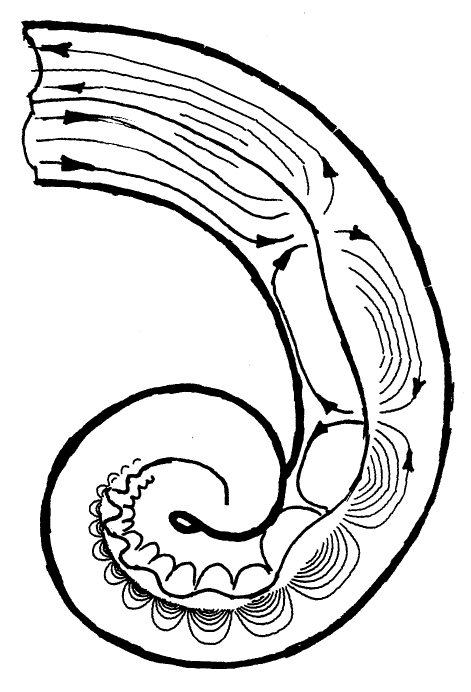
\includegraphics[height=3in]{../lec18/Cochlea_Traveling_Wave.png}}
  \begin{tiny}
    Dick Lyon, public domain image, 2007.
    \url{https://en.wikipedia.org/wiki/File:Cochlea_Traveling_Wave.png}
  \end{tiny}
\end{frame}

\begin{frame}
  \centerline{\includegraphics[height=3in]{../lec18/exp/gammatone_filterbank.png}}
\end{frame}
     
\begin{frame}
  \frametitle{The Power of Filtered White Noise}

  Suppose that $h[n]$ is the auditory filter centered at frequency $f_c$ (in Hertz), and
  \[
  y[n]=h[n]\ast x[n]
  \]
  where $x[n]$ is white noise.  What's the power of the signal $y[n]$?
  \begin{align*}
    \frac{1}{N}\sum_n y^2[n] &= \frac{1}{F_s}\int_{-F_s/2}^{F_s/2} R_{yy}\left(\frac{2\pi f}{F_s}\right) df\\
    &= \frac{1}{F_s}\int_{-F_s/2}^{F_s/2} R_{xx}\left(\frac{2\pi f}{F_s}\right)|H(f)|^2 df
  \end{align*}
  So the expected power is
  \[
  E\left[\frac{1}{N}\sum_n y^2[n]\right] = \frac{\sigma^2}{F_s}\int_{-F_s/2}^{F_s/2} |H(f)|^2 df
  \]
  \ldots so, OK, what is $\int_{-F_s/2}^{F_s/2} |H(f)|^2 df$?
\end{frame}

%%%%%%%%%%%%%%%%%%%%%%%%%%%%%%%%%%%%%%%%%%%%
\section[Bandwidth]{What is the Bandwidth of the Auditory Filters?}
\setcounter{subsection}{1}

\begin{frame}
  \frametitle{Bandwidth}

  \centerline{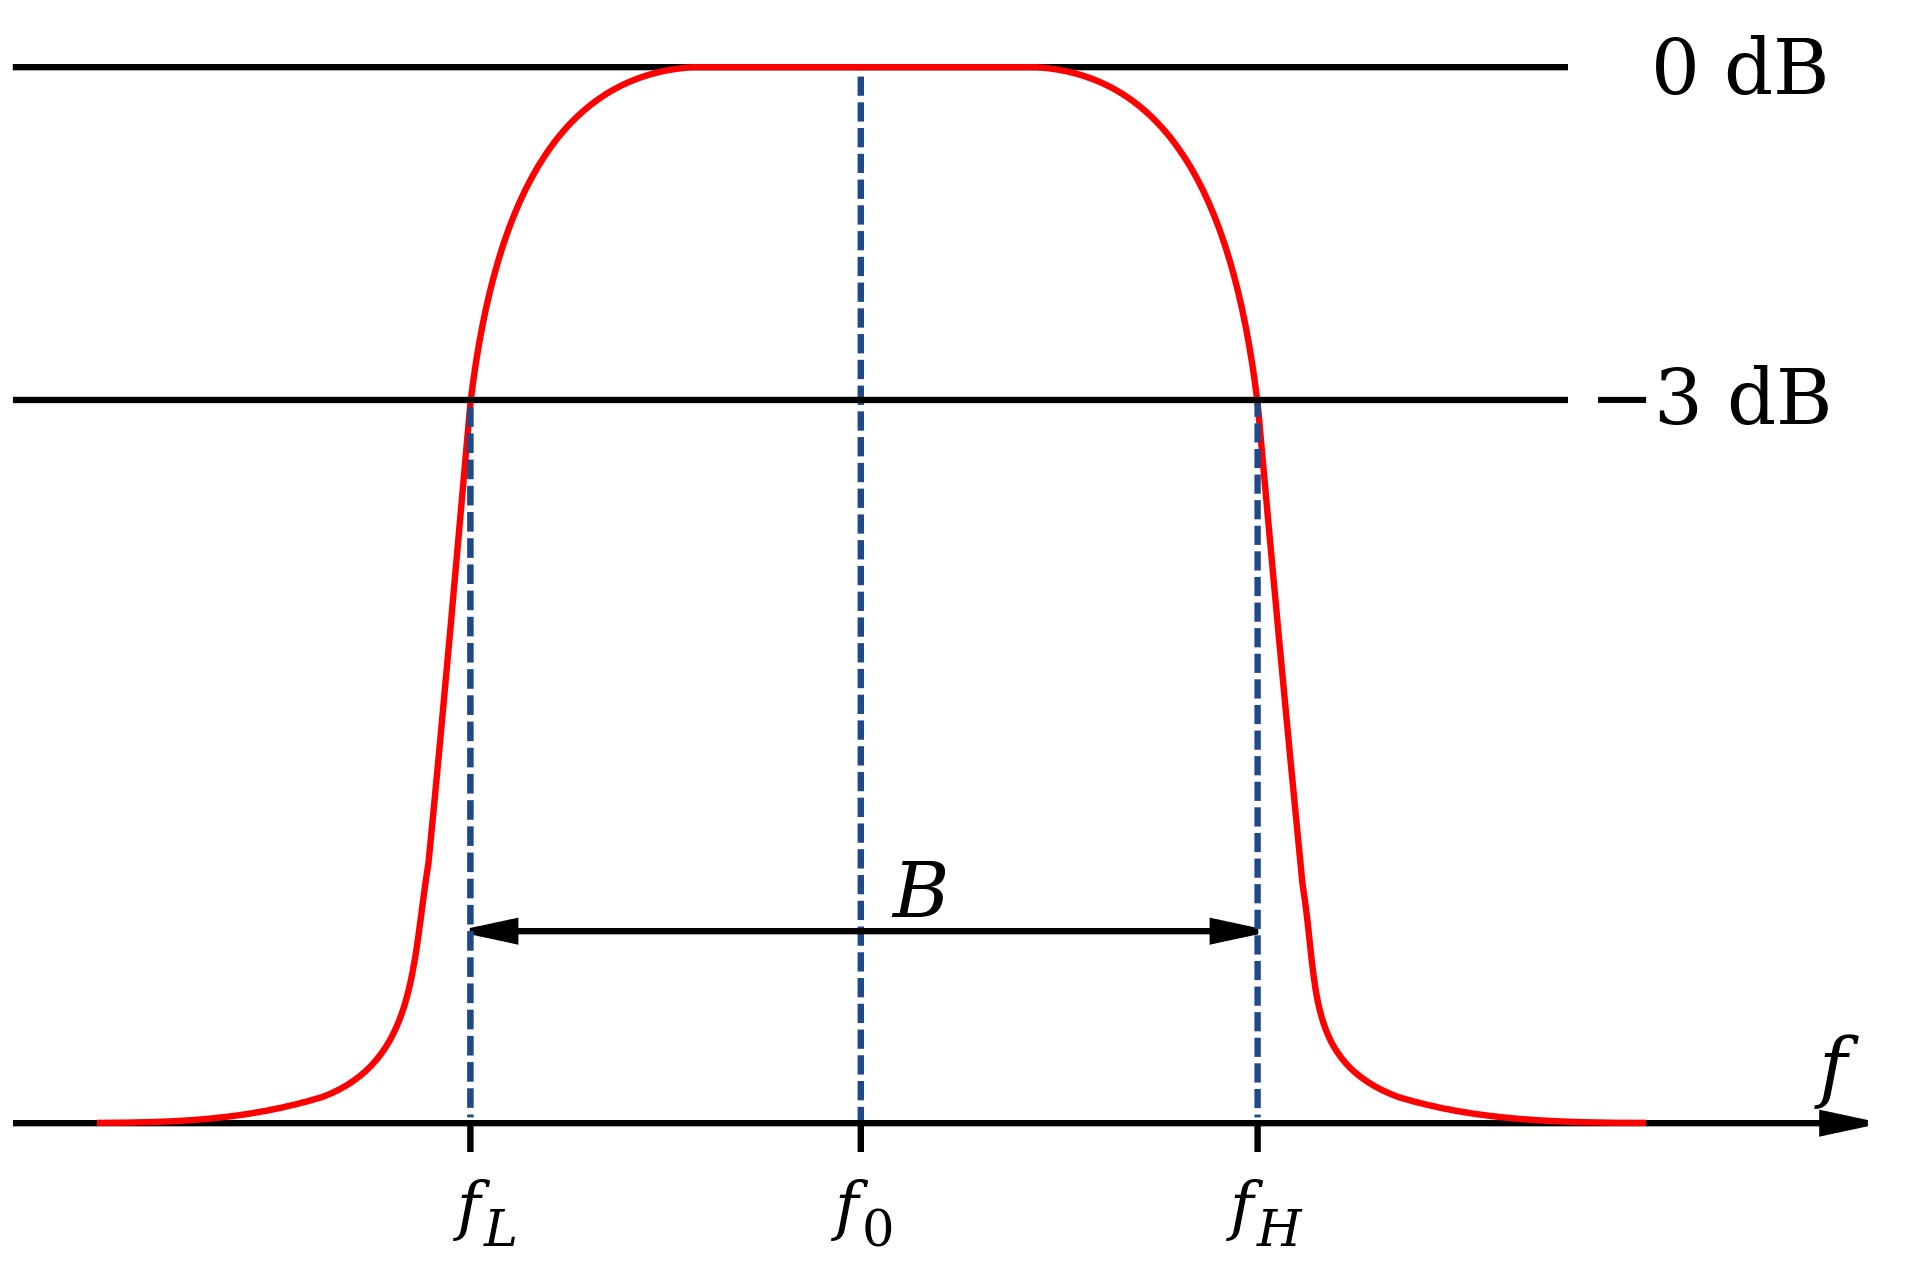
\includegraphics[height=2in]{Bandwidth_2.png}}
  \begin{tiny}
    By InductiveLoad, public domain image,
    \url{https://commons.wikimedia.org/wiki/File:Bandwidth_2.svg}
  \end{tiny}
\end{frame}

\begin{frame}
  \frametitle{Equivalent rectangular bandwidth}

  Let's make the simplest possible assumption: a rectangular filter,
  centered at frequency $f_c$, with bandwidth $b$:
  \[
  H(f) = \begin{cases}
    1 & f_c-\frac{b}{2} < f <f_c+\frac{b}{2}\\
    1 & f_c-\frac{b}{2} < -f < f_c+\frac{b}{2}\\
    0 & \mbox{otherwise}
  \end{cases}
  \]
  That's useful, because it makes Parseval's theorem very easy:
  \[
  \frac{\sigma^2}{F_s}\int_{-F_s/2}^{F_s/2} |H(f)|^2 df = \left(\frac{2b}{F_s}\right)\sigma^2
  \]
\end{frame}
  
\begin{frame}
  \frametitle{Reminder: Fletcher's Model of Masking}

  Fletcher proposed the following model of hearing in noise:
  \begin{enumerate}
  \item The human ear pre-processes  the audio using a bank of bandpass filters.
  \item The power of the noise signal, in the 
    bandpass filter centered at frequency $f_c$, is $N_{f_c}$.
  \item The power of the noise+tone is $N_{f_c}+T_{f_c}$.
  \item If there is {\bf\em any} band, $k$, in which
    $\frac{N_{f_c}+T_{f_c}}{N_{f_c}}>\mbox{threshold}$, then the tone is audible.
    Otherwise, not.
  \end{enumerate}
\end{frame}

\begin{frame}
  \frametitle{The ``Just Noticeable Difference'' in Loudness}

  First, let's figure out what the threshold is.  Play two white noise
  signals, $x[n]$ and $y[n]$.  Ask listeners which one is louder.

  The ``just noticeable difference'' is the difference in loudness at
  which 75\% of listeners can correctly tell you that $y[n]$ is louder than $x[n]$:
  \[
  \mbox{JND} = 10\log_{10}\left(\sum_n y^2[n]\right) - 10\log_{10}\left(\sum_n x^2[n]\right)
  \]
  It turns out that the JND is very close to 1dB, for casual
  listening, for most listeners.  So Fletcher's masking criterion becomes:
  \begin{itemize}
    \item If there is {\bf\em any} band, $l$, in which
      $10\log_{10}\left(\frac{N_{f_c}+T_{f_c}}{N_{f_c}}\right)>1\mbox{dB}$, then
      the tone is audible.  Otherwise, not.
  \end{itemize}
\end{frame}

\begin{frame}
  \frametitle{Fletcher's Model, for White Noise}

  \begin{enumerate}
  \item The human ear pre-processes  the audio using a bank of bandpass filters.
  \item The power of the noise signal, in the  filter centered at $f_c$, is $N_{f_c}=2b\sigma^2/F_s$.
  \item The power of the noise+tone is $N_{f_c}+T_{f_c}$.
  \item If there is any band in which
    $10\log_{10}\left(\frac{N_{f_c}+T_{f_c}}{N_{f_c}}\right)>1\mbox{dB}$, then
    the tone is audible.  Otherwise, not.
  \end{enumerate}
  \ldots next question to solve.  What is the power of the tone?
\end{frame}

\begin{frame}
  \frametitle{What is the power of a tone?}

  A pure tone has the formula
  \[
  x[n] = A\cos\left(\omega_0 n+\theta\right),~~~\omega_0=\frac{2\pi}{N_0}
  \]
  Its power is calculated by averaging over any integer number of
  periods:
  \[
  T_{f_c} = \frac{1}{N_0}\sum_{n=0}^{N_0-1} A^2\cos^2\left(\omega_0 n+\theta\right) = \frac{A^2}{2}
  \]
\end{frame}

\begin{frame}
  \frametitle{Power of a filtered tone}

  Suppose $y[n]=h[n]\ast x[n]$.  Then
  \[
  y[n] = A|H(\omega_0)|\cos\left(\omega_0 n+\theta+\angle H_{f_c}(\omega_0)\right)
  \]
  And it has the power
  \[
  T_{f_c} = \frac{1}{2}A^2 |H(\omega_0)|^2
  \]
  If we're using rectangular bandpass filters, then
  \[
  T_{f_c} = \begin{cases}
    \frac{A^2}{2} & f_c-\frac{b}{2}< f_0 <f_c+\frac{b}{2}\\
    \frac{A^2}{2} & f_c-\frac{b}{2} < -f < f_c+\frac{b}{2} \\
    0 & \mbox{otherwise}
  \end{cases}
  \]
\end{frame}

\begin{frame}
  \frametitle{Fletcher's Model, for White Noise}

  The tone is audible if there's some filter centered at $f_c\approx f_0$ (specifically,
  $f_c-\frac{b}{2}< f_0 <f_c+\frac{b}{2}$)  for which:
  \[
  1\mbox{dB} < 10\log_{10}\left(\frac{N_{f_c}+T_{f_c}}{N_{f_c}}\right)
  = 10\log_{10}\left(\frac{\frac{2b\sigma^2}{F_s}+\frac{A^2}{2}}{\frac{2b\sigma^2}{F_s}}\right)
  \]
  Procedure: Set $F_s$ and $\sigma^2$ to some comfortable listening
  level.  In order to find the bandwidth, $b$, of the auditory filter centered at $f_0$,
  \begin{enumerate}
  \item Test a range of different levels of $A$.
  \item Find the minimum value of $A$ at which listeners can report
    ``tone is present'' with 75\% accuracy.
  \item From that, calculate $b$.
  \end{enumerate}
\end{frame}

\begin{frame}
  \frametitle{Equivalent rectangular bandwidth (ERB)}

  Here are the experimental results: The frequency resolution of your
  ear is better at low frequencies!  In fact, the dependence is
  roughly linear (Glasberg and Moore, 1990):
  \[
  b \approx 0.108 f + 24.7
  \]
  These are often called (approximately) constant-Q filters, because
  the quality factor is
  \[
  Q = \frac{f}{b} \approx 9.26
  \]
  The dependence of $b$ on $f$ is not quite linear.  A more precise
  formula is given in (Moore and Glasberg, 1983) as:
  \[
  b = 6.23\left(\frac{f}{1000}\right)^2 + 93.39\left(\frac{f}{1000}\right)+28.52
  \]
\end{frame}

\begin{frame}
  \frametitle{Equivalent rectangular bandwidth (ERB)}

  \centerline{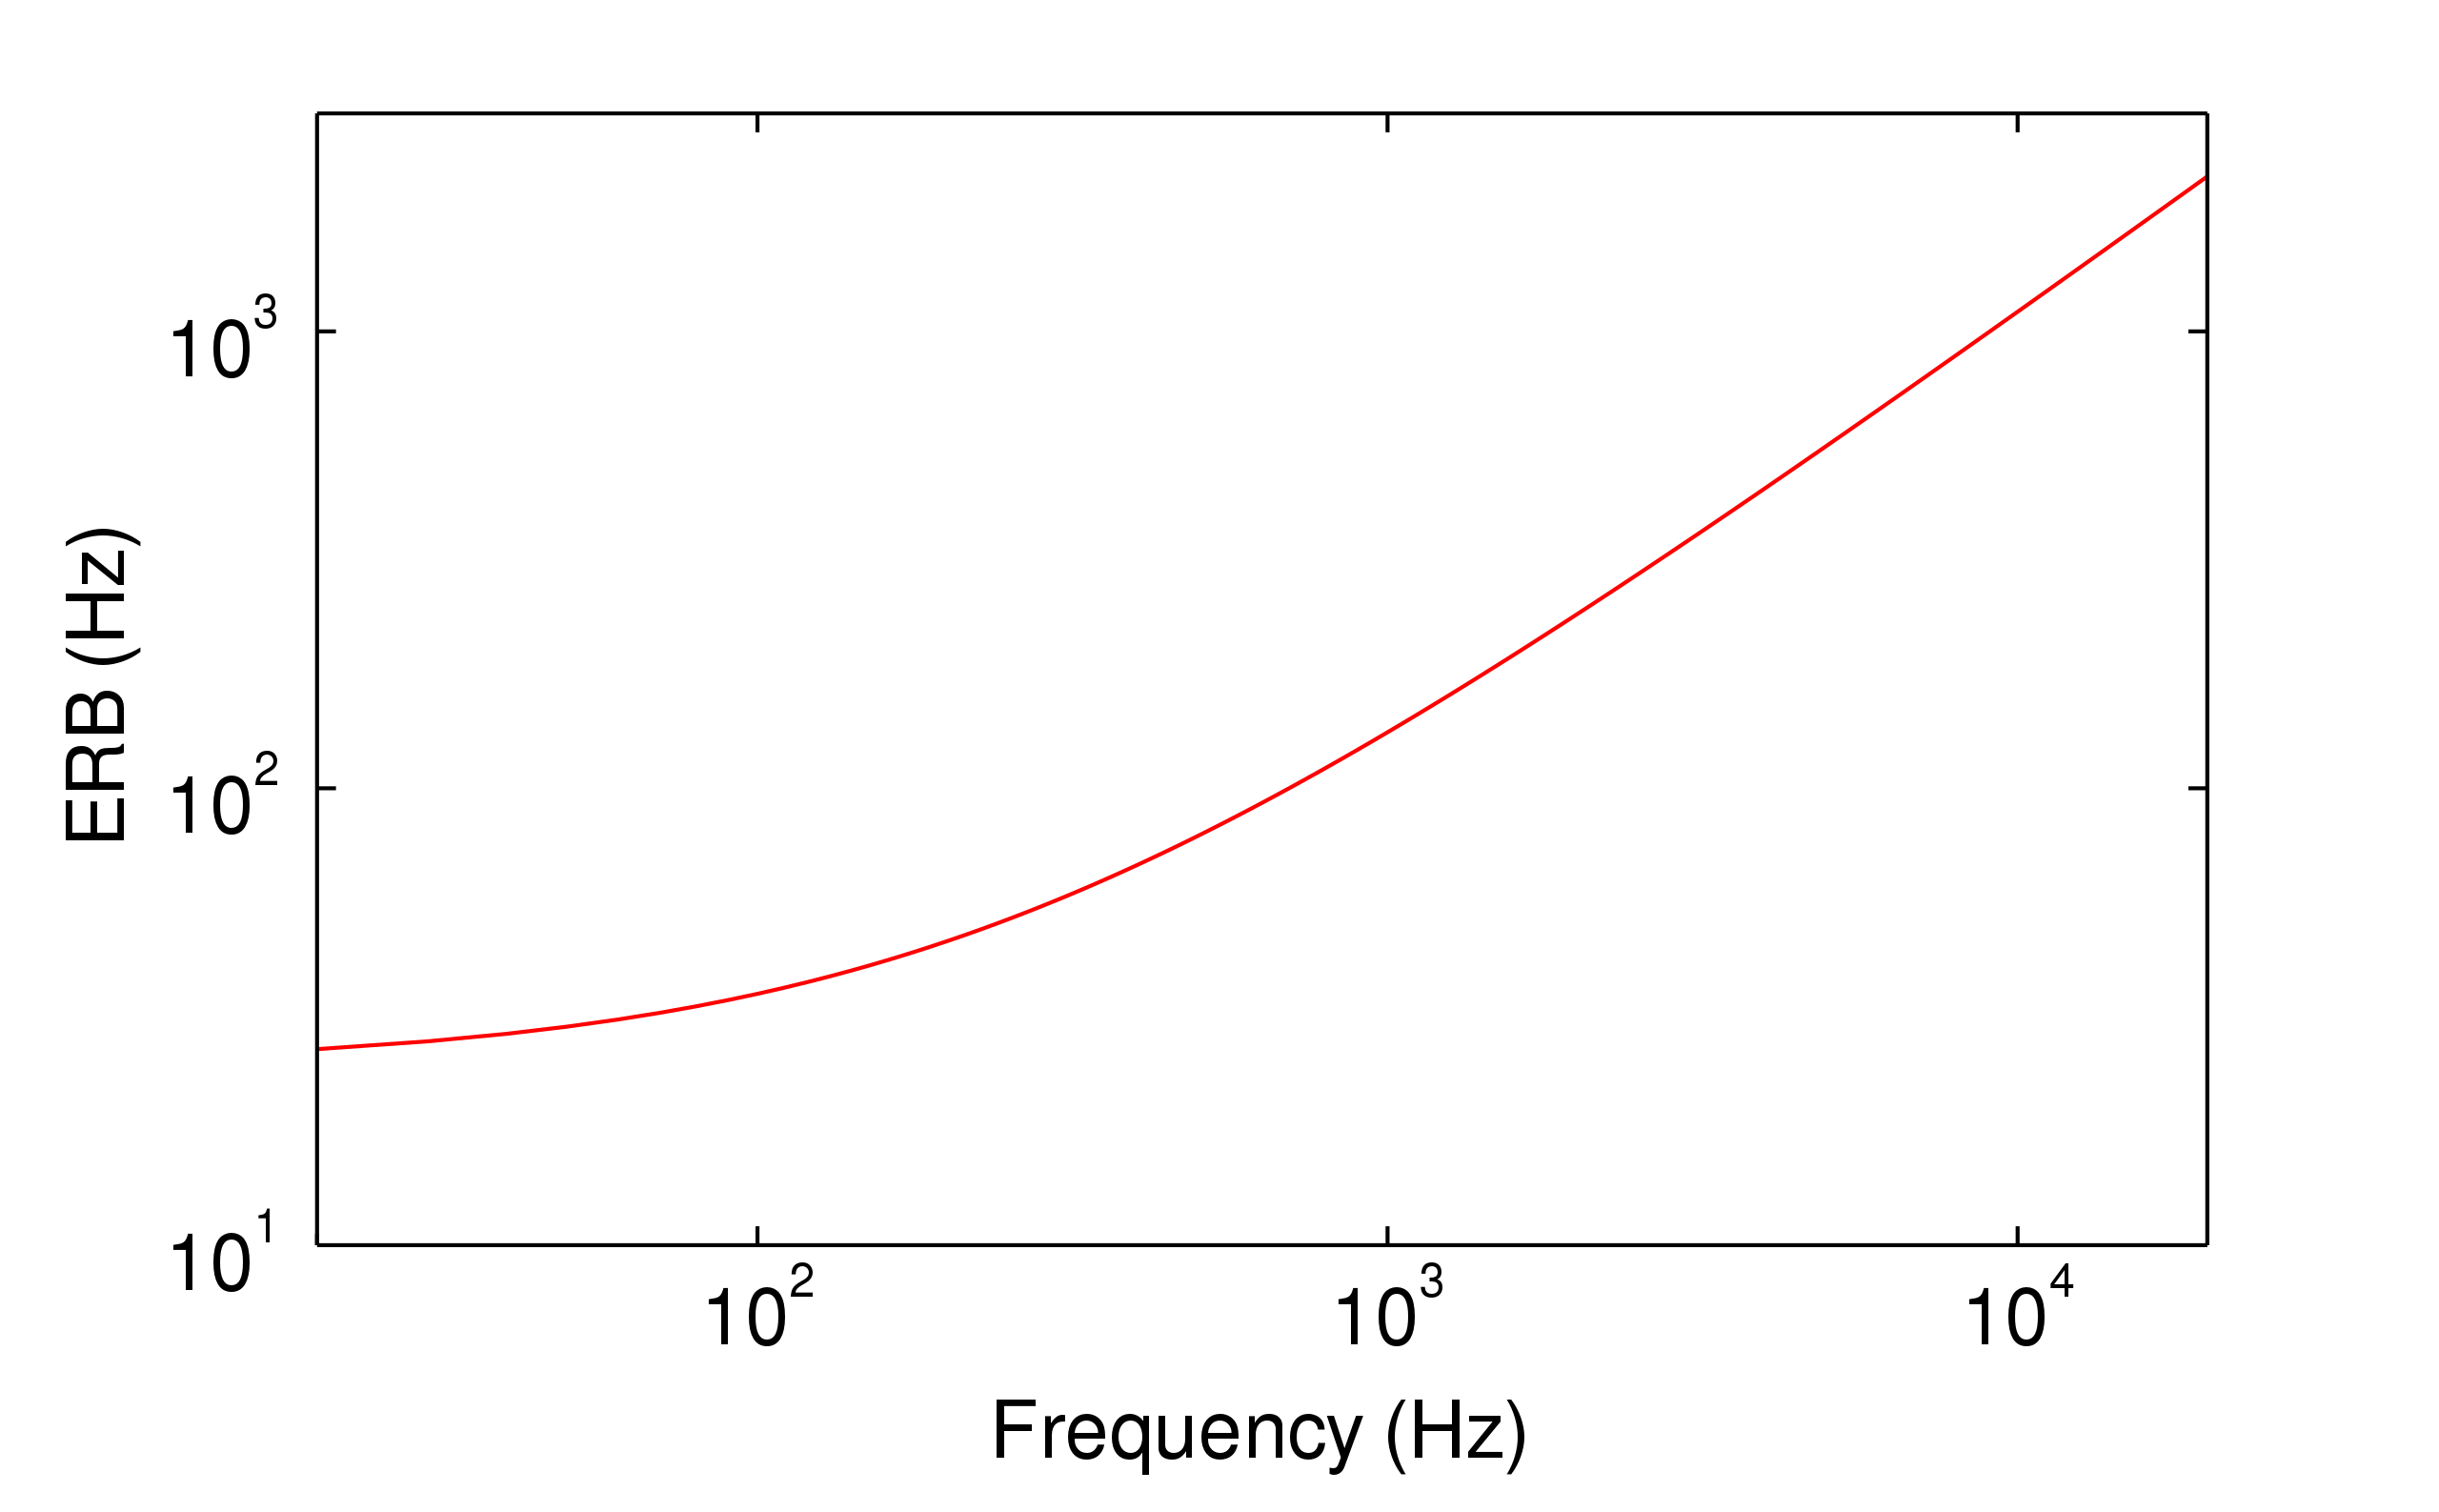
\includegraphics[height=2in]{2560px-ERB_vs_frequency.png}}
  \begin{tiny}
    By Dick Lyon, public domain image 2009,
    \url{https://commons.wikimedia.org/wiki/File:ERB_vs_frequency.svg}
  \end{tiny}
\end{frame}

%%%%%%%%%%%%%%%%%%%%%%%%%%%%%%%%%%%%%%%%%%%%%%%%%%%%%%%%
\section[Bandstop]{Auditory-Filtered Other Noises}
\setcounter{subsection}{1}

\begin{frame}
  \frametitle{What happens if we start with bandstop noise?}

  \centerline{\includegraphics[height=2.5in]{../lec03/exp/tone_bandstop_powerspectrum.png}}
\end{frame}

\begin{frame}
  \frametitle{The power of bandstop noise}

  Suppose $y[n]$ is a bandstop noise: say, it's been zeroed out between $f_2$ and $f_3$:
  \[
  E\left[R_{yy}(\omega)\right] = \begin{cases}
    0 & f_2 < |f| < f_3\\
    \sigma^2 &  \mbox{otherwise}
  \end{cases}
  \]
  Parseval's theorem gives us the energy of this noise:
  \begin{align*}
    E\left[\frac{1}{N}\sum_{n=0}^{N-1}y^2[n]\right]
    &=\frac{1}{F_s}\int_{-F_s/2}^{F_s/2} R_{yy}(\omega)d\omega\\
    & \sigma^2\left(1-\frac{2(f_3-f_2)}{F_s}\right)
  \end{align*}
  If $f_3-f_2\ll \frac{F_s}{2}$, then the power of this noise is
  almost as large as the power of a white noise signal.
\end{frame}

\begin{frame}
  \frametitle{Bandstop noise power $\approx$ White noise power}

  \centerline{\includegraphics[height=1.5in]{../lec03/exp/tone_white_waveform.png}}
  \centerline{\includegraphics[height=1.5in]{../lec03/exp/tone_bandstop_waveform.png}}
\end{frame}

\begin{frame}
  \frametitle{Auditory-filtered bandstop noise}

  Now let's filter $y[n]$ through an auditory filter:
  \[
  z[n] = y[n]\ast h[n]
  \]
  where, again, let's assume a rectangular auditory filter, and let's assume that the
  whole bandstop region lies inside the auditory filter, so that
  \[
  f_c-\frac{b}{2} < f_3 < f_2 < f_c+\frac{b}{2}
  \]
  Then we have
  \[
  E\left[R_{zz}(f)\right] = E\left[R_{yy}(f)\right]|H(f)|^2 = \begin{cases}
    \sigma^2 & f_c-\frac{b}{2} < |f| < f_2\\
    \sigma^2 & f_3 < |f| < f_c+\frac{b}{2} \\
    0 & \mbox{otherwise}
  \end{cases}
  \]
  This is nonzero only in two tiny frequency bands:  $f_c-\frac{b}{2} < |f| < f_2$, and
  $f_3 < |f| < f_c+\frac{b}{2}$.
\end{frame}

\begin{frame}
  \frametitle{Auditory-filtered bandstop noise}

  \centerline{\includegraphics[height=2.5in]{../lec03/exp/gtfiltered_bandstop_powerspectrum.png}}
\end{frame}

\begin{frame}
  \frametitle{Tiny power spectrum $\Rightarrow$ tiny waveform energy}

  \centerline{\includegraphics[height=1.5in]{../lec03/exp/gtfiltered_bandstop_waveform.png}}
  \centerline{\includegraphics[height=1.5in]{../lec03/exp/gtfiltered_white_waveform.png}}
\end{frame}

%%%%%%%%%%%%%%%%%%%%%%%%%%%%%%%%%%%%%%%%%%%%
\section[Shape]{What is the Shape of the Auditory Filters?}
\setcounter{subsection}{1}

\begin{frame}
  \frametitle{Lowpass noise}

  Patterson (1974) measured the shape of the auditory filter using
  lowpass noise, i.e., noise with the following spectrum:

  \[
  R_{xx}(f)  =\begin{cases}
  \sigma^2 & -f_1 < f<f_1\\ 0&\mbox{otherwise}
  \end{cases}
  \]
\end{frame}
  
\begin{frame}
  \frametitle{Lowpass-filtered noise}

  \centerline{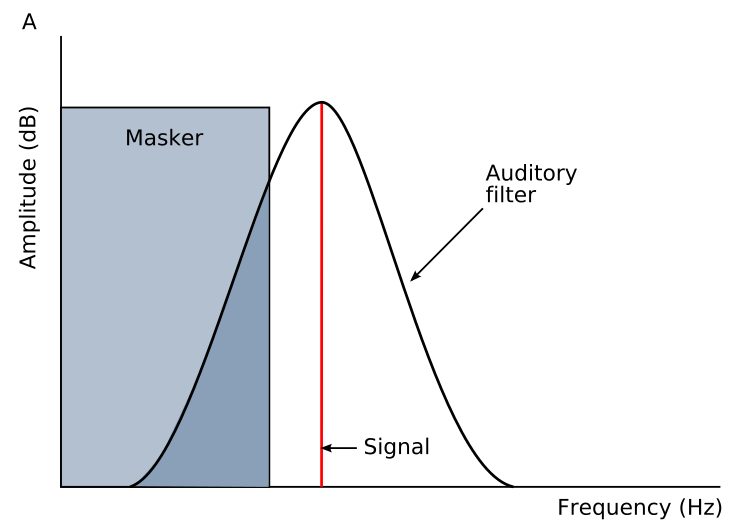
\includegraphics[height=2.5in]{Off_F_listening.png}}
  \begin{tiny}
    By Dave Dunford, public domain image 1010,
    \url{https://en.wikipedia.org/wiki/File:Off_F_listening.svg}
  \end{tiny}
\end{frame}

\begin{frame}
  \frametitle{Lowpass noise}

  Patterson (1974) measured the shape of the auditory filter using
  lowpass noise, i.e., noise with the following spectrum:

  \[
  R_{xx}(f)  =\begin{cases}
  \sigma^2 & -f_1 < f<f_1\\ 0&\mbox{otherwise}
  \end{cases}
  \]
  The power of a lowpass filtered noise, as heard through
  an auditory filter $H(f)$ centered at $f_c$, is
  \[
  N(f_c,f_1)= \frac{1}{F_s}\int_{-F_s/2}^{F_s/2} R_{xx}(f) |H(f)|^2 df
  = \frac{\sigma^2}{F_s}\int_{-f_1}^{f_1} |H(f)|^2 df
  \]
  Turning that around, we get a formula for $|H(f)|^2$ in terms of the
  power, $N(f_c,f_1)$, that gets passed through the filter:
  \[
  |H(f)|^2=\left(\frac{F_s}{2\sigma^2}\right)
  \frac{dN(f_c,f_1)}{df_1}
  \]
\end{frame}


\begin{frame}
  \frametitle{The power of lowpass noise}

  Suppose that we have a tone at $f_0\approx f_c$, and we raise its
  amplitude, $A$, until it's just barely audible.  The relationship between the
  tone power and the noise power, at the JND amplitude, is
  \[
  10\log_{10}\left(\frac{N(f_c,f_1)+0.5A^2}{N(f_c,f_1)}\right) = 1~~~\Rightarrow~~~
  N(f_c,f_1)= \frac{0.5A^2}{10^{1/10}-1}
  \]
  So if we measure the minimum tone amplitude that is audible, as a  function
  of $f_c$ and $f_1$, then we get 
  \[
  |H(f)|^2 = \left(\frac{1.93 F_s}{\sigma^2}\right)
  \frac{dA(f_c,f_1)}{df_1}
  \]
  \ldots so the shape of the auditory filter is the derivative, with respect to
  cutoff frequency, of the smallest audible power of the tone at $f_c$.
\end{frame}

\begin{frame}
  \frametitle{Symmetric filters}

  Using the method on the previous slide, Patterson showed that the
  auditory filter shape varies somewhat depending on loudness, but the
  auditory filter centered at $f_0$ is pretty well approximated as
  \[
  |H(f)|^2 = \frac{1}{(b^2+(f-f_0)^2)^4}
  \]
\end{frame}

\begin{frame}
  \frametitle{What is the inverse transform of a symmetric filter?}

  \[
  |H(f)|^2 = \frac{1}{(b^2+(f-f_0)^2)^4}
  \]
  Patterson suggested analyzing this as
  \[
  |H(f)|^2 = \frac{1}{(b^2+(f-f_0)^2)^4}= \left||G(f)|^2\right|^4
  \]
  where
  \[
  |G(f)|^2 = \frac{1}{b^2+(f-f_0)^2}
  \]
\end{frame}

\begin{frame}
  \frametitle{What is the inverse transform of $|G(f)|$?}

  First, let's just consider the filter
  \[
  |G(f)|^2 = \frac{1}{b^2+(f-f_0)^2}
  \]
  The only causal filter with this frequency response is the basic
  second-order resonator filter,
  \[
  G(f) = \frac{2\pi}{2\pi (b-j(f-f_0))}
  \]
  \ldots which is the Fourier transform ($G(f)=\int g(t)e^{-j2\pi ft}dt$) of 
  \[
  g(t) = \begin{cases}
    2\pi e^{-2\pi (b-jf_0)t} & t>0\\
    0 & t<0
  \end{cases}
  \]
\end{frame}

\begin{frame}
  \frametitle{What does $g(t)$ look like?}

  The real part of $g(t)$ is $e^{-2\pi bt}\cos(2\pi f_0t)u(t)$, which is
  shown here:
  \centerline{\includegraphics[height=2in]{dampedsine.png}}
  \begin{tiny}
    By LM13700, CC-SA3.0,
    \url{https://commons.wikimedia.org/wiki/File:DampedSine.png}
  \end{tiny}
\end{frame}

\begin{frame}
  \frametitle{What does $|G(f)|$ look like?}

  $|G(f)|$ looks like this (the frequency response of a standard second-order
  resonator filter). It's closest to the olive-colored one:

  \centerline{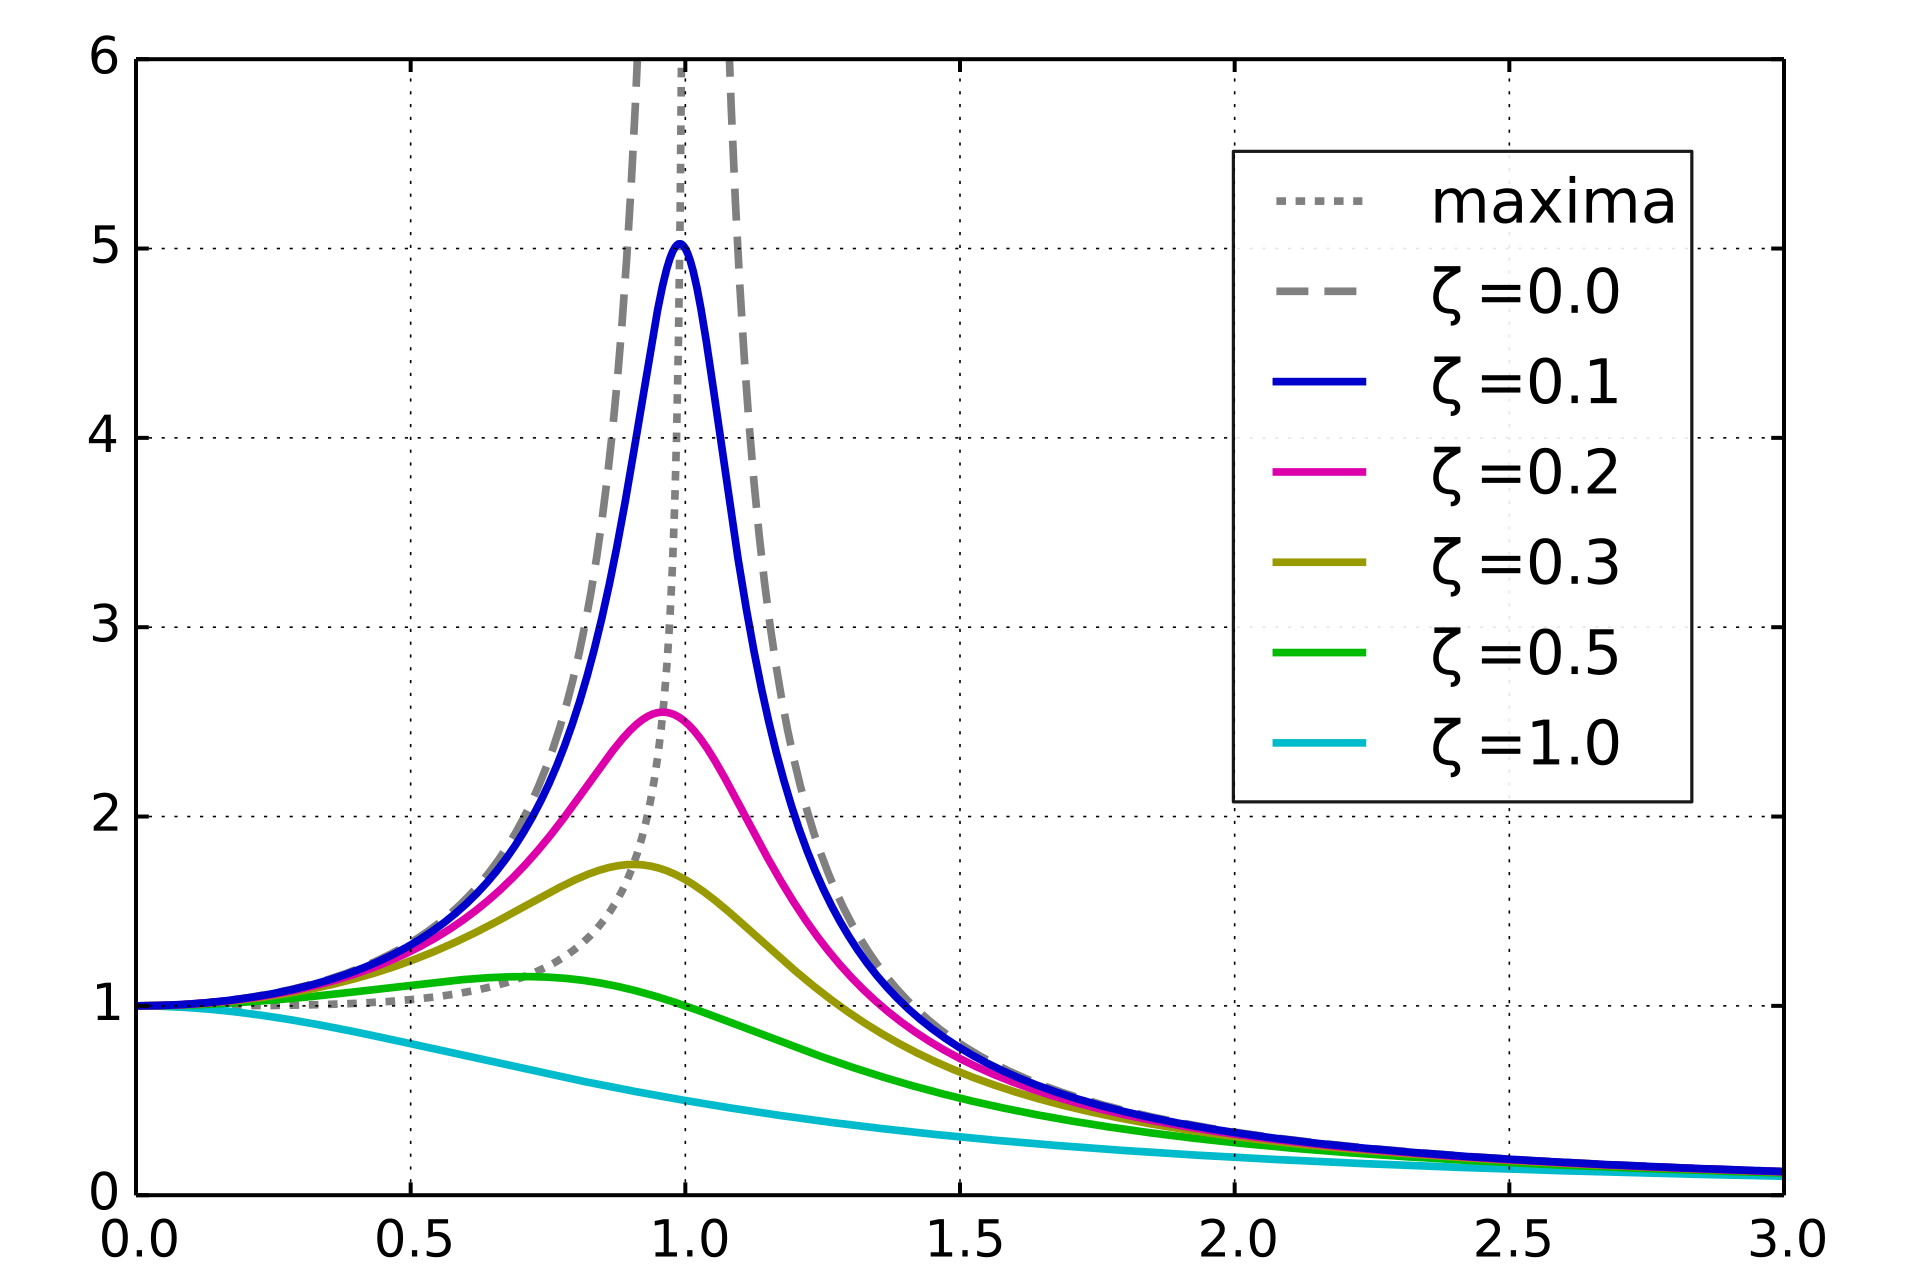
\includegraphics[height=2in]{Mplwp_resonance_zeta_envelope.png}}
  \begin{tiny}
    By Geek3, Gnu Free Documentation License,
    \url{https://commons.wikimedia.org/wiki/File:Mplwp_resonance_zeta_envelope.svg}
  \end{tiny}
\end{frame}

\begin{frame}
  \frametitle{From $G(f)$ to $H(f)$}

  Patterson suggested analyzing $H(f)$ as
  \[
  |H(f)|^2 = \frac{1}{(b^2+(f-f_0)^2)^4}= \left||G(f)|^2\right|^4
  \]
  which means that
  \[
  h(t) = g(t)\ast g(t)\ast g(t)\ast g(t)
  \]
  So what is $g(t)\ast g(t)$?
\end{frame}

\begin{frame}
  \frametitle{The self-convolution of an exponential is  a gamma}

  Let's first figure out what is $g(t)\ast g(t)$, where 
  \[
  g(t)=e^{-at}u(t),~~~a=2\pi (b-jf_0)
  \]
  We can write it as
  \begin{align*}
    g(t)\ast g(t) &= \int_0^t e^{-a\tau} e^{-a(t-\tau)} d\tau\\
    &= e^{-at} \int_0^t e^{-a\tau} e^{+a\tau} d\tau\\
    &= te^{-at} u(t)
  \end{align*}
  Repeating that process, we get
  \[
  g(t)\ast g(t)\ast g(t)\ast g(t) \propto t^3 e^{-at}u(t)
  \]
\end{frame}

\begin{frame}
  \frametitle{The Gammatone Filter}

  Patterson proposed that, since $h(t)$ is obviously real-valued, we
  should model it as
  \[
  H(f) = \left(\frac{1}{b + j(f-f_0)}\right)^n + \left(\frac{1}{b + j(f+f_0)}\right)^n
  \]
  Whose inverse transform is a filter called a {\bf gammatone filter}
  (because it looks like a gamma function, from statistics, multiplied
  by a tone):
  \[
  h(t) \propto t^{n-1} e^{-2\pi bt}\cos(2\pi f_0 t)u(t)
  \]
  where, in this case, the order of the gammatone is $n=4$.
\end{frame}

\begin{frame}
  \frametitle{The Gammatone Filter}

  The top frame is a white noise, $x[n]$.  The middle frame is a
  gammatone filter at $f_c=1000$Hz, with a bandwidth of $b=128$Hz.
  The bottom frame is the filtered noise $y[n]$.

  \centerline{\includegraphics[height=2in]{../lec03/exp/gtfiltered_white_waveform.png}}
\end{frame}
  
